\chapter{RNA Base-Pairs}
\label{basepairs} 
\bibliographystyle{nar}
\section{Canonical and Noncanonical Base-pairs}
As  shown   in  Figure  \ref{fig:saenger28},  there   can  be  various
base-pairing patterns between heterocyclic  bases in nucleic acids due
to the  variety of possible  hydrogen bonding interactions.   The most
prevalent hydrogen  bonding pattern  in nucleic acids  is that  of the
canonical  Watson-Crick  (WC)  base-pair.   Other  possible  patterns
besides the WC one are known as non-canonical base-pairs and are more
common in  RNA than in DNA.   We used the  3DNA \cite{lu2003} software
package  to find  all base-pairs  in  a non-redundant  dataset of  RNA
structures  obtained by X-ray  crystallography with  resolution better
than 3.5  \AA~ downloaded from the  protein data bank  (PDB).  We also
constrained our search to helical regions, which are defined as having
three  consecutive base-pairs  or more  which need  not  be covalently
bonded by the  sugar-phosphate backbone between consecutive base-pairs
\cite{olson2009}.

\begin{table}[htbp]
\begin{center}
\begin{tabular}{|l|c|r|r|r|r|}
\hline
RNA Type & \multicolumn{1}{p{2cm}|}{Number of Structures} & \multicolumn{1}{c|}{G} &
\multicolumn{1}{c|}{C} & \multicolumn{1}{c|}{A} &
\multicolumn{1}{c|}{U} \\ \hline 
small helices & 78 & 891 & 753 & 404 & 442 \\ \hline
drug-RNA & 36 & 932 & 862 & 365 & 433 \\ \hline
protein-RNA & 207 & 4001 & 3457 & 1771 & 1731 \\ \hline
protein-tRNA & 9 & 175 & 155 & 98 & 87 \\ \hline
rRNA & 13 & 3866 & 2949 & 1939 & 1785 \\ \hline
tRNA & 13 & 205 & 159 & 124 & 112 \\ \hline
ribozyme & 113 & 2434 & 2086 & 1438 & 1150 \\ \hline
Total & 469 & \multicolumn{1}{c|}{12504} & \multicolumn{1}{c|}{10421} & \multicolumn{1}{c|}{6139} & \multicolumn{1}{c|}{5740} \\ \hline
\end{tabular}
\caption{Description   of  the   type   of  RNA   structures  in   the
  non-redundant  dataset  at  less  than 3.5  \AA~(for  base-pairs  in
  helices of 3 base-pairs or more).}
\label{tab:dbase}
\end{center}
\end{table}

Our dataset is  non-redundant in the sense that  from the main source
of RNA structural information, which is the ribosome, we used only one
of the  available structures  per organism, that  is, one for  each of
\textit{Deinococus   radiodurans},   \textit{Haloarcula  marismortui},
\textit{Escherichi          coli},         and         \textit{Thermus
  thermophilus}. Table~\ref{tab:dbase}  shows in detail  the number of
bases per  RNA type in  our dataset. It's  interesting to see  that in
general the content of  G and C, is higher than that  of A and U which
might be due to the  highest overall stability of G$\cdot$C base-pairs
against A$\cdot$U base-pairs.

In Table  \ref{tab:bpcomp} we show  all possible base-pairs  formed by
unmodified nucleotides in our dataset,  it's clear from this table that
the G$\cdot$C  and A$\cdot$U base-pairs  dominate widely the  space of
possible  RNA base-pairs  in helical  regions  making up  80\% of  all
base-pairs,  and  if  we  only  count those  that  form  canonical  WC
base-pairs (9500  G$\cdot$C, and 3069  A$\cdot$U), they make  up about
73\% of all base-pairs in helical regions.

As will  be show later (Table~\ref{tab:seven}),  a considerable amount
of A$\cdot$U's  pair in the  Hoogsteen fashion. Few of  these examples
form    U$\cdot$A$\cdot$U   triplets   containing    a   WC    and   a
Hoogsteen \footnote{Hoogsteen base-pairs  are illustrated by structure
  XXIII  of  the Saenger  classification  of  base-pairs  as shown  in
  Figure~\ref{fig:saenger28}} base-pair in RNA helical regions.

\begin{table}[htbp]
\begin{center}
\begin{tabular}{|c|c|c|c|c|}
\hline
A    &      G    &      C    &      U    &      B$_{\text{1}}$$\cdot$B$_{\text{2}}$ \\ \hline
384  &    980    &    313    &   3975    &      A  \\ \hline
     &    128    &   9913    &   1282    &      G  \\ \hline
     &           &     63    &    103    &      C  \\ \hline
     &           &           &    187    &      U  \\ \hline
\end{tabular}
\caption{Composition  of  base-pairs  in  non-redundant  dataset  with
  resolutions better  than 3.5  \AA~ (for base-pairs  in helices  of 3
  base-pairs or more).  Note that 9500 out of  9913 G$\cdot$C and 3069
  out of 3975 A$\cdot$U are canonical WC base-pairs.}
\label{tab:bpcomp}
\end{center}
\end{table}

\subsection{RNA Base-Pairs Classification}
We classified the RNA base-pairs  in our dataset using three criteria.
(1) The Leontis-Westhof  edge classification scheme \cite{leontis1998}
which is based on the  identification of three major interacting edges
for hydrogen-bond  formation called WC  edge (W), Hoogsteen  edge (H),
and Sugar edge (S).  (2) The rotational and translational base-pairing
rigid-body parameters, shear,  stretch, stagger, buckle, propeller and
opening.  (3)  The location of  base-pairs in helices, that  is, their
location  in ``intact''  covalently bonded  sugar-phosphate backbones,
and in  the ends  of ``quasi-continuous'' helices  with breaks  in the
sugar-phosphate backbone.

In  out dataset  we  find that  $\sim$90\%  of the  base-pairs in  RNA
helices will form base-pairs in one of seven possible hydrogen-bonding
types, these  were found to  be canonical WC G$\cdot$C  and A$\cdot$U,
and the  non-canonical G$\cdot$U wobble,  sheared G$\cdot$A, Hoogsteen
A$\cdot$U, WC type G$\cdot$A, and U$\cdot$U wooble base-pair. Detailed
results  showing how  these  seven major  RNA  base-pairing types  are
classified  according to  various schemes,  and the  details  of their
hydrogen-bond  distances  is  given  in Table~\ref{tab:seven}  and  in
Figure~\ref{fig:pairs}

\begin{sidewaystable}
\begin{center}
\begin{tabular}{|c c|c c|c|c|c c|c|}
\hline
Base-pair & & Hydrogen bonds &  & Sign & Saenger & Leontis-Westhof & &
Number \\
\hline
\hline
\multicolumn{9}{|l|}{Canonical} \\
\hline
G$\cdot$C & Watson-Crick & N2-H$\cdots$O2 & 2.79(0.17) & - & XIX & cis
 & W/W & 9500$_{\text{x0.90}}$ \\
 & & O6$\cdots$H-N4 & 2.92(0.18) & & & & &  \\
 & & N1-H$\cdots$N3 & 2.89(0.13) & & & & &  \\
\hline
A$\cdot$U & Watson-Crick & N1$\cdots$H-N3 & 2.84(0.14) & - & XX & cis
& W/W & 3069$_{\text{x0.93}}$ \\
 & & N6-H$\cdots$O4 & 2.97(0.18) & & & & &  \\
\hline
\multicolumn{9}{|l|}{Non-canonical} \\
\hline
G$\cdot$U & Wobble & N1-H$\cdots$O2 & 2.79(0.16) & - & XXVIII & cis
 & W/W & 1049$_{\text{x0.69}}$ \\
 & & O6$\cdots$H-N3 & 2.85(0.16) & & & & &  \\
\hline
G$\cdot$A & Sheared & N2-H$\cdots$N7 & 2.89(0.17) & + & XI & trans
 & H/S & 509$_{\text{x0.59}}$ \\
 & & N3$\cdots$H-N6 & 3.03(0.18) & & & & &  \\
\hline
A$\cdot$U & Hoogsteen & N6-H$\cdots$O2 & 2.91(0.21) & + & XXIII & trans
 & H/W & 354$_{\text{x0.71}}$ \\
 & & N7$\cdots$H-N3 & 2.90(0.17) & & & & &  \\
\hline
G$\cdot$A & Watson-Crick & N1-H$\cdots$N1 & 2.84(0.17) & - & VIII & cis
 & W/W & 185$_{\text{x0.85}}$ \\
 & & O6$\cdots$H-N6 & 2.91(0.20) & & & & &  \\
\hline
U$\cdot$U & Wobble & O2$\cdots$H-N3 & 2.95(0.24) & - & XVI & cis
 & W/W & 141$_{\text{x0.54}}$ \\
 & & N3$\cdots$H-O4 & 2.87(0.15) & & & & &  \\
\hline
\end{tabular}
\caption{Seven  main base-pairing  types in  RNA helical  dataset. The
  first  column uses  the  Gutell and  collaborators nomenclature  for
  base-pairs, column  two shows the prefered  hydrogen bonding pattern
  for each base-pair, column  four gives the Saenger classification as
  in Figure \ref{fig:saenger28}, column five gives the Leontis-Westhof
  edge  classification obtained  trough the  RNAVIEW program,  and the
  last column gives the total  number of identified base-pairs of each
  category and the  percentage of those which comply  exactly with the
  hydrogen-bonding pattern of column two.}
\label{tab:seven}
\end{center}  
\end{sidewaystable}  

\begin{figure}[htbp]
\centering
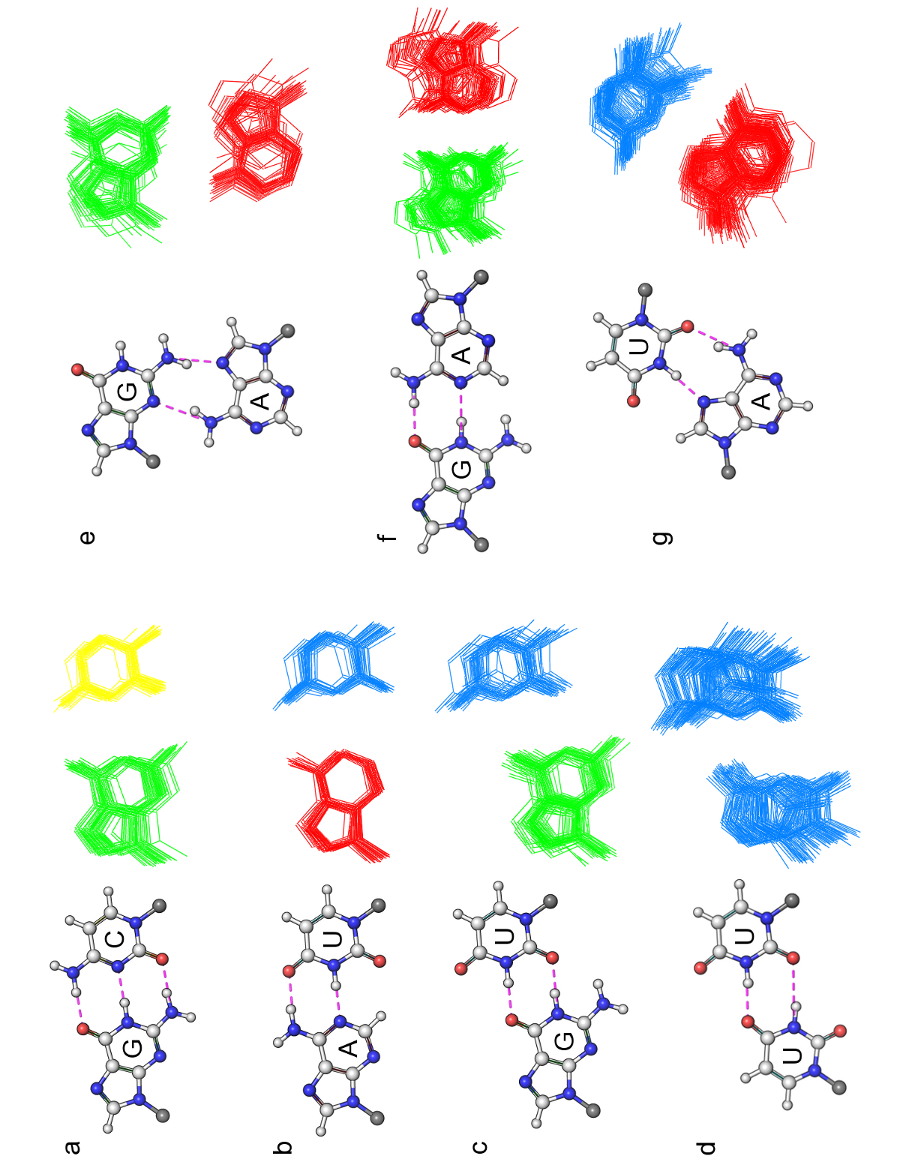
\includegraphics[angle=-90, scale=0.6]{Chapter3/sevenpairs.png}
\caption{Seven   most   prominent  pairs   in   RNA  helical   regions
  dataset.  The  images  to  the  left  of  each  base-pair  show  the
  hydrogen-bond  connectivity  as magenta  colored  dashed lines.  The
  rigth  side   images  on   each  base-pair  representation   show  a
  superposition of the base-pairs  in our helical dataset, centered in
  the middle base triad reference frame. }
\label{fig:pairs}
\end{figure}

\subsection{Base-Pairs in Helical Regions}
Our classification also includes the location of base-pairs in helical
regions, that is, whether they are  in the interior or in the terminal
ends     of     ``intact''     or     ``quasi-continuous''     helical
regions.  Figure~\ref{fig:helregxin}  illustrates  the  two  types  of
helical regions  mentioned. In (a) an  ``intact'' helical region
is depicted and in (b) a ``quasi-continuos'' helical region is shown.

\begin{figure}
\centering
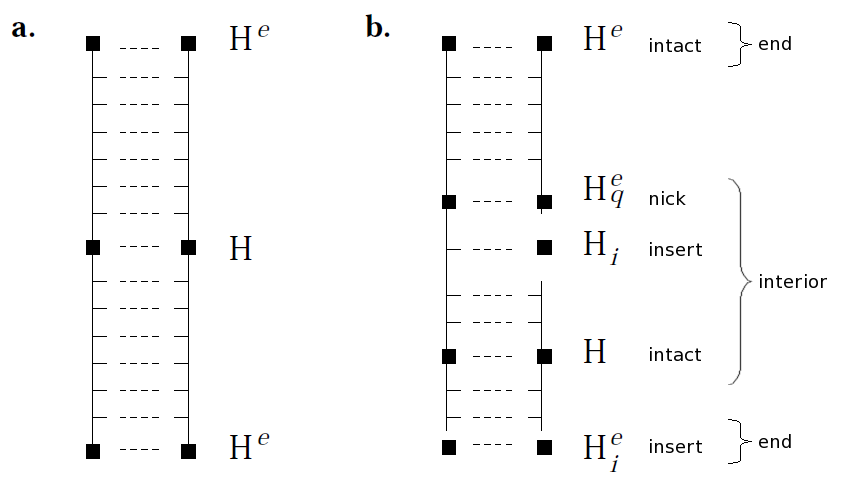
\includegraphics[scale=0.4]{Chapter3/helcontext.png}
\caption{(a)  Intact  and  (b)  quasi-continuous  helical  regions  in
  RNA. Image kindly provided by Dr. Yurong Xin.}
\label{fig:helregxin}
\end{figure}  

The results obtained from  the classification of base-pairs in helical
regions  are  shown in  Table~\ref{tab:helcontext}.   We  see that  in
particular  the   A$\cdot$U  Hoogsteen  pair  (A$\cdot$U$_{\text{H}}$)
stands out as  being present mainly as an  insert \footnote{Similar to
  the way  intercalating ligands (intercalators)  insert themselves in
  DNA.} in helical regions, sometimes  in nicked regions and rarely in
intact   ones.   Now,   for  the   G$\cdot$A   Watson-Crick-like  pair
(G$\cdot$A$_{\text{WC}}$) we see the  inverse situation to that of the
A$\cdot$U  Hoogsteen pair,  that is,  it rarely  occurs as  an insert,
prefering to be  in nicks, and sometimes in  intact regions, a similar
situation     happens    with     the    sheared     G$\cdot$A    pair
(G$\cdot$A$_{\text{s}}$),  which is also  rare as  an insert  and it's
mainly found in intact regions, and sometimes in nicks.  The canonical
WC G$\cdot$C base-pair is two times more likely to occur at the end of
helical  regions than  the other  canonical base-pair  A$\cdot$U.  The
helical context of  the G$\cdot$U wobble pair (G$\cdot$U$_{\text{w}}$)
is quite  similar to  that of the  canonical base-pairs,  more closely
resembling  the  context  of  G$\cdot$C$_{\text{WC}}$,  than  that  of
A$\cdot$U$_{\text{WC}}$, it differentiates from them on being slightly
more  prevalent  in  nicked regions  than  any  of  the two,  and  the
G$\cdot$U wobble pair (G$\cdot$U$_{\text{w}}$) is present in a similar
context  to that  of the  canonical A$\cdot$U,  more commonly  seen in
interior  regions than in  ends.  It  is interesting  to see  that the
G$\cdot$C$_{\text{WC}}$ has a helical context practically identical to
the  one given for  all base-pairs.   The mean  length of  the helical
domains   in  the   dataset   is   11  bp   as   show  in   supplement
Figure~\ref{fig:hellength}  which indicates  that the  canonical A-RNA
conformation is predominant and is most likely maintained by canonical
WC pairs which constitute 73\% of all base-pairs.

\begin{table}[htbp]
\begin{center}
\begin{tabular}{|c|c|c|c|c|c|c|c|c|}
\hline
Helical context & \multicolumn{8}{c|}{Base-pair} \\
\hline
 & All & G$\cdot$C$_{\text{WC}}$ & A$\cdot$U$_{\text{WC}}$ &
G$\cdot$U$_{\text{w}}$ & G$\cdot$A$_{\text{s}}$ &
A$\cdot$U$_{\text{H}}$ & G$\cdot$A$_{\text{WC}}$ &
U$\cdot$U$_{\text{w}}$  \\
\hline
\multicolumn{9}{|c|}{Interior} \\
\hline
Intact &  0.62 & 0.62 & 0.75 & 0.63 & 0.34 & 0.05 & 0.25 & 0.74 \\
Nick   &  0.20 & 0.20 & 0.16 & 0.26 & 0.25 & 0.29 & 0.66 & 0.13 \\
Insert &  0.02 & 0.01 & 0.01 & 0.00 & 0.00 & 0.42 & 0.01 & 0.03 \\
\hline
\multicolumn{9}{|c|}{Ends} \\
\hline
Intact &  0.13 & 0.15 & 0.07 & 0.10 & 0.33 & 0.05 & 0.06 & 0.10 \\
Insert &  0.02 & 0.01 & 0.01 & 0.01 & 0.05 & 0.19 & 0.02 & 0.00 \\
\hline
\end{tabular}
\caption{Distribution in helical context of the seven most abundant
  base-pairs in our RNA helical regions dataset.}
\label{tab:helcontext}
\end{center}
\end{table}

\section{Deformability of Base-Pairs}
Figure   \ref{fig:pairs}  shows   a  visual   representation   of  the
deformability of the seven  most predominant base-pairs in RNA helical
regions. The overlapping structures for each base-pair are centered in
the  middle base  triad  (see appendix  \ref{appendix_1a} detail).  In
Table  \ref{tab:bppar}  we  have  collected  the  averages  and  their
corresponding  standard deviations  for the  rigid-body  parameters of
base-pairs, along with a
deformability score,  which is obtained  by the product of  the square
roots  of  the  eigenvalues  of the  base-step  parameters  covariance
matrix, such  volume score is  refered to as  accesible conformational
volume, also the root-mean-square deviation (rmsd) of the superimposed
structures in given.

The first  observation which stands out from  Table \ref{tab:bppar} is
that  non-canonical  base-pairs   are  clearly  more  deformable  than
canonical WC base-pairs.   This larger deformability in non-canonicals
comes mainly  from the in-plane  parameters, that is,  Shear, Stretch,
and Opening, whereas the  out-of-plane parameters Stagger, Buckle, and
Propeller are somewhat  comparable to those of the  less deformable WC
base-pairs, that is, there  is more deformability in non-canonicals at
the level of  hydrogen-bonding interactions, and less at  the level of
stacking interactions which constrain  the base-pairs to planarity. In
accordance with  this, the  variability of hydrogen-bond  distances is
also   greater  in   non-canonical   base-pairs  as   seen  in   Table
\ref{tab:seven}. Another  fact that confirms  this greater variability
is  that the  fraction  of  base-pairs which  comply  strictly to  the
hydrogen bonding pattern of  Table \ref{tab:seven} is much smaller for
non-canonicals as seen  in the last column. For  example, if one looks
at the amount of canonical  WC G$\cdot$C which complies to the binding
pattern shown  as given in  column three, then  one has 90  percent of
G$\cdot$C's  binding in  such pattern,  whereas  for the  case of  the
U$\cdot$U wobble  base-pair, only  54 percent of  base-pairs associate
following the  O2$\cdots$H-N3 and N3-  H$\cdots$O4 interacting pattern
strictly.    What's  occurring   with  the   additional  non-canonical
base-pairs  which  are  not  included in  the  hydrogen-bond  distance
averages  is that  they  are  either ``melting'',  that  is, they  are
forming less  hydrogen bonds  in order to  pair, or, they  are forming
different types of heavy atoms bridges mediated by hydrogen.


A direct
quantification of conformational volume by looking at the partitioning
of  the covariational  space for  base-pair parameters  cannot  give a
direct 

the distribution
of the covariation 


trough use  of  the space  of
base-pair parameters does not strictly give a 


The  units  of  the  rigid-body  parameters,  i.e.,  angles
expressed  in  degrees and  distances  in  Ångstrom units,  complicate
assessment of the relative  deformabilities of different base pairs in
terms of the  accessible conformational volume V.

A  larger value of V
does not  necessarily indicate  greater overall spatial  movement. The
root-mean-square  deviations  of  the  superimposed images  yield  the
following  deformability   rankings:  U$\cdot$U$_{w}$  (0.74   \AA)  >
G$\cdot$A$_{WC}$  (0.54 \AA)  $\approx$ G$\cdot$A$_{s}$  (0.50  \AA) >
G$\cdot$U$_{w}$  (0.45  \AA) $\approx$  A$\cdot$U$_{H}$  (0.43 \AA)  >
G$\cdot$C$_{WC}$ (0.38  \AA) $\approx$ A$\cdot$U$_{WC}$  (0.36 \AA), a
slightly  different ordering  from  the computed  values  of V  (Table
3).

Surprisingly,  some of the  most deformable base pairs  occur with
greater likelihood  in the duplex interior e.g.,  the U$\cdot$U wobble
pair, and some of the more  rigid pairs occur at ``nicks'' or resemble
drug-like inserts,  e.g., the  A$\cdot$U Hoogsteen pair.

The relative
stiffness of  the latter arrangements  comes at no surprise  given the
preferential crystallization of free A  and U in Hoogsteen pairs [26].

Finally,  the  non-canonical  base  pairs  have  unique  deformability
profiles  partially  reflective of  the  pattern  of interaction.

For
example,  G  and  U tend  to  fluctuate  via  Shear along  the  short,
hydrogenbonded axis of the G$\cdot$U wobble  pair, but G and A tend to
slide  past one another  via Stretch  along the  long axis  of contact
between sheared  G$\cdot$A pairs.

The A$\cdot$U Hoogsteen  bases move
along both  axes and  rotate in the  base-pair plane via  Opening. The
major fluctuations of the  U$\cdot$U wobble and G$\cdot$A Watson-Crick
pairs entail Shear and Opening.

\begin{sidewaystable}[htbp]
\begin{center}
\begin{tabular}{|c|c|c|c|c|c|c|c|c|}
\hline
Base-pair & \multicolumn{7}{c|}{Rigid-body parameters} \\
\hline
 & Shear (\AA) & Stretch (\AA) & Stagger (\AA) & Buckle (deg) &
Propeller (deg) & Opening (deg) & V (deg$^{\text{3}}$
\AA$^{\text{3}}$) & rmsd \\
\hline
G$\cdot$C$_{\text{WC}}$ & -0.20 (0.41) & -0.15 (0.17) & -0.04 (0.40) & -3.4 (8.4)  &  -8.7  (8.5) &  0.5  (4.5)  & 6.5   & 0.38\\
A$\cdot$U$_{\text{WC}}$ &  0.04 (0.34) & -0.14 (0.15) &  0.04 (0.39) & -0.3 (8.4)  &  -9.0  (8.7) &  0.9  (5.2)  & 6.4   & 0.36\\
G$\cdot$U$_{\text{w}}$  & -2.11 (0.84) & -0.52 (0.27) & -0.04 (0.43) & -0.1 (8.2)  &  -7.4  (7.5) & -0.6  (6.9)  & 25.1  & 0.45\\
G$\cdot$A$_{\text{s}}$  &  6.78 (0.23) & -4.40 (0.55) &  0.14 (0.52) &  1.5 (11.0) &  -3.2  (9.1) & -5.3  (8.2)  & 27.2  & 0.50\\
A$\cdot$U$_{\text{H}}$  & -4.06 (0.80) & -1.92 (0.84) &  0.07 (0.61) & -0.4 (7.3)  &   1.0 (10.8) & -95.1 (17.4) & 25.9  & 0.43\\
G$\cdot$A$_{\text{WC}}$ & -2.34 (0.59) & -1.63 (0.31) & -0.09 (0.47) &  0.6 (8.8)  & -11.1  (7.8) & -0.2  (17.4) & 49.8  & 0.74\\
U$\cdot$U$_{\text{w}}$  &  0.00 (0.64) &  1.52 (0.40) & -0.29 (0.41) &  7.8 (10.8) & -10.8  (9.6) & -17.2 (13.5) & 86.2  & 0.54\\
\hline
\end{tabular}
\caption{Rigid-body base-pair parameters, their standard deviations
  and their conformational accesible volume score.}
\label{tab:bppar}
\end{center}
\end{sidewaystable}




\section{Clustering of Yurong's Classification}

\bibliography{biblio}

